% !TEX root = ../main.tex  

\chapter{Introduction}\label{ch:intro}
In this report we will be looking at how strategies of the Iterated Prisoners Dilemma (IPD) can be `countered' or `worked' in order to give a better overall score for a player on the other side of the game.
We will look into explicit sequences which should be played for $1$ vs $1$ games of length 200 to gain the highest score per turn upon the games conclusion.
These sequences will then be compared and contrasted to understand how some opponents could be grouped together even though they have no structure in common.

Our concept of `working' a strategy is more fitting in this research as we will be looking into boosting the score or our player, which in most cases (due to the nature of the IPD) will also boost the score of our opponent.
`working' also has a better real world interpretation than `countering' as the real goal of increasing the score for our player is to generate as many Cooperation moves to Defect against without consequences as possible.

This paper assumes a basic knowledge of game theory and how to model a normal form game.
The IPD game itself is described in Section~\ref{sec:iteratedPrisonersDilemma} and the real world research is discussed in Chapter~\ref{ch:literature}.


\section{The Prisoners Dilemma and Its Iterated Form}\label{sec:iteratedPrisonersDilemma}
\begin{center}
    \itshape~Two members of a criminal gang are arrested and imprisoned.
    Each prisoner is in solitary confinement with no means of communicating with the other.
    The prosecutors lack sufficient evidence to convict the pair on the principal charge.
    They hope to get both sentenced to a year in prison on a lesser charge. Simultaneously, the prosecutors offer each prisoner a bargain.
    Each prisoner is given the opportunity either to: betray the other by testifying that the other committed the crime, or to cooperate with the other by remaining silent.
\end{center}

The Prisoners Dilemma is a normal form game in the space $\mathbb{R}^{{2\times 2}^2}$ with utility matrices for the row and column player as follows:
$$
    A=\begin{pmatrix}R & S\\ T & P\end{pmatrix}\quad
    B=\begin{pmatrix}R & T\\ S & P\end{pmatrix}
$$
with the following constraints (scoring highly is good):
$$T>R>P>S \qquad \vert \qquad 2R>T+S$$
These constraints model the above story with the following definitions:
\begin{itemize}
    \item $T$ --- Temptation, the utility for successfully tricking your opponent to confess.
    \item $R$ --- Reward, by staying silent with your opponent you receive the reward.
    \item $P$ --- Punishment, if both you and your opponent confess you'll receive the punishment
    \item $S$ --- Sucker, if you confess but your opponent stays silent you're a sucker.
\end{itemize}
This ensures that the game reaches some fundamental dilemmas, and hence its name.
Do you \textbf{Cooperate} and risk being taken advantage of by your opponent, first row or column.
Or do you \textbf{Defect} and hope your opponent stays silent, second row or column.
We will be using the following utilities for this paper.
$$
    A=\begin{pmatrix}3 & 0 \\ 5 & 1\end{pmatrix}\quad
    B=\begin{pmatrix}3 & 5 \\ 0 & 1\end{pmatrix}
$$    
From a game theoretic point of view it can be seen that there exists a strongly dominant strategy for both the row and column players; to defect each move.
This however doesn't reflect on the iterated version of the game where repetition can allow for higher overall scores if players are coordinated and cooperate with one another.

We will be looking into the iterated form of the game which, simply put, is just a series of games back to back. 
Players do not know what their opponent will play on any given turn, but can have an indefinite amount of time between turns.
Players can algorithmically, stochastically or using a combination of the two decide on their next move.
The number of turns is often provided beforehand, but doesn't need to be, and the overall score of the game is normalised to by this to allow for comparisons between games of different length.

\section{Brief Task Overview}\label{sec:briefOverview}
This document will be be looking at the creation of sequences to beat given opponents in The Iterated Prisoners Dilemma.
Analysis will be focused on looking into just the single opponent use case, but the idea of designing a sequence for a tournament for a given number of opponents is a potential follow on to this work.
Our task is as follows:

Problem:
\begin{center}
    \itshape~When playing a given Iterated Prisoners Dilemma strategy, \(O\), as an opponent, what is the best ordered solution sequence of moves, \(S\), to play in order for us to obtain the highest possible average score per move across the game.
\end{center}

For example an opponent known as Tit For Tat, which cooperates on its first move and the copies your last move on subsequent moves, will have a solution sequence of moves that are all cooperation apart from the last.
This is an obvious example and a simple strategy to calculate for, the ultimate goal of this investigation is to look into every strategy as defined in the Axelrod Library.
These are listed in appendix Section~\ref{apndx:opponents} and definitions can be found in the axelrod codebase\cite{axelrodproject}.


\section{Machine Learning \& Computer Intelligence}\label{sec:machineLearningAndcomputerIntelligence}
Machine Learning is a field of computer science that has existed since the first computers have been around.
Most famously the questions posed by Alan Turing in 1950~\cite{turing1950computing} asks `can machines think', a question that has been refined and analysed to this day.
The field of computer intelligence is rich in its complexities and has recently been making breakthroughs~\cite{knight2017alphaZeroMIT} on topics which would traditionally be considered `thinking'.
Along with this, recently there has also been record levels of funding~\cite{chui2017artificial} put in to companies which operate in this field, producing results in areas that would usually seem `solved'.

\subsection{Genetic Algorithms}\label{subsec:geneticAlgorithms}
This report will cover one of the forms of machine learning called genetic algorithms (GAs).
Genetic Algorithms fall under a branch of machine learning called evolutionary feature selection algorithms.
More generally, genetic algorithms are put into a class of unsupervised reinforcement learning algorithms.
These are techniques of using genetic algorithms for generating solutions to problems that typically revolve around heuristically improving members of a population who represent these solutions.
The concept of a genetic algorithm, and more generally an evolutionary algorithm, comes from nature;
like nature we create a survival of the fittest selection~\cite{darwin2009origin} competition to evaluate a population then kill off the weakest members.
After this cull we create offspring from the most successful population or introduce new members from a predefined source.
This process is then repeated until we stop it, or forever in the case of nature.

We say a genetic algorithm is structured in the following way.
Given a population, \(P\), each with unique genes (genes and member properties are interchangeable), and a number of generations, \(G\in \mathbb{N}\), the algorithm will create \(G\) cycles of scoring and potentially removing each of the members of the population, \(p_i \in P\).
It does this by using a mapping from a member of the population to an ordered set, for example \(f(p_i)\mapsto \mathbb{R},\ p_i \in P\).
This function, \(f\), is defined beforehand in a way which describes the goal of our investigation.
Defining a cut-off or bottleneck \(b<|P|\), such that on conclusion of completing any cycle, the top \(b\) ranking members by score can be kept and the rest discarded.
By doing this we are saving the more successful candidates allowing us to rebuild the population using a series of crossovers and mutations (and possibly introducing new members into the population) with the genes which were successful.

\begin{itemize}
    \item Crossovers take in 2 members of the population and return a new member based on some parameters of the 2 `parents'.
    For example, our crossover takes the first half of a sequence from one and the second half from the other, merging them to form the third.
    \item Mutations allow a (possibly targeted\footnote{For example using intuition and targeting specific genes, or allowing another algorithm to improve the targeting of this meta function.}) change in a single member of the population.
    A mutation has 2 parameters, a potency \(M_p\in \mathbb{R}>0\) and a frequency \(M_f\in [0,1]\).
    \(M_p\) describes how strong the mutation is, the higher it is the larger change to the member occurs.
    \(M_f\) explains the percentage of how many members of the population are mutated.
\end{itemize}

\begin{figure}[ht]
    \centering
    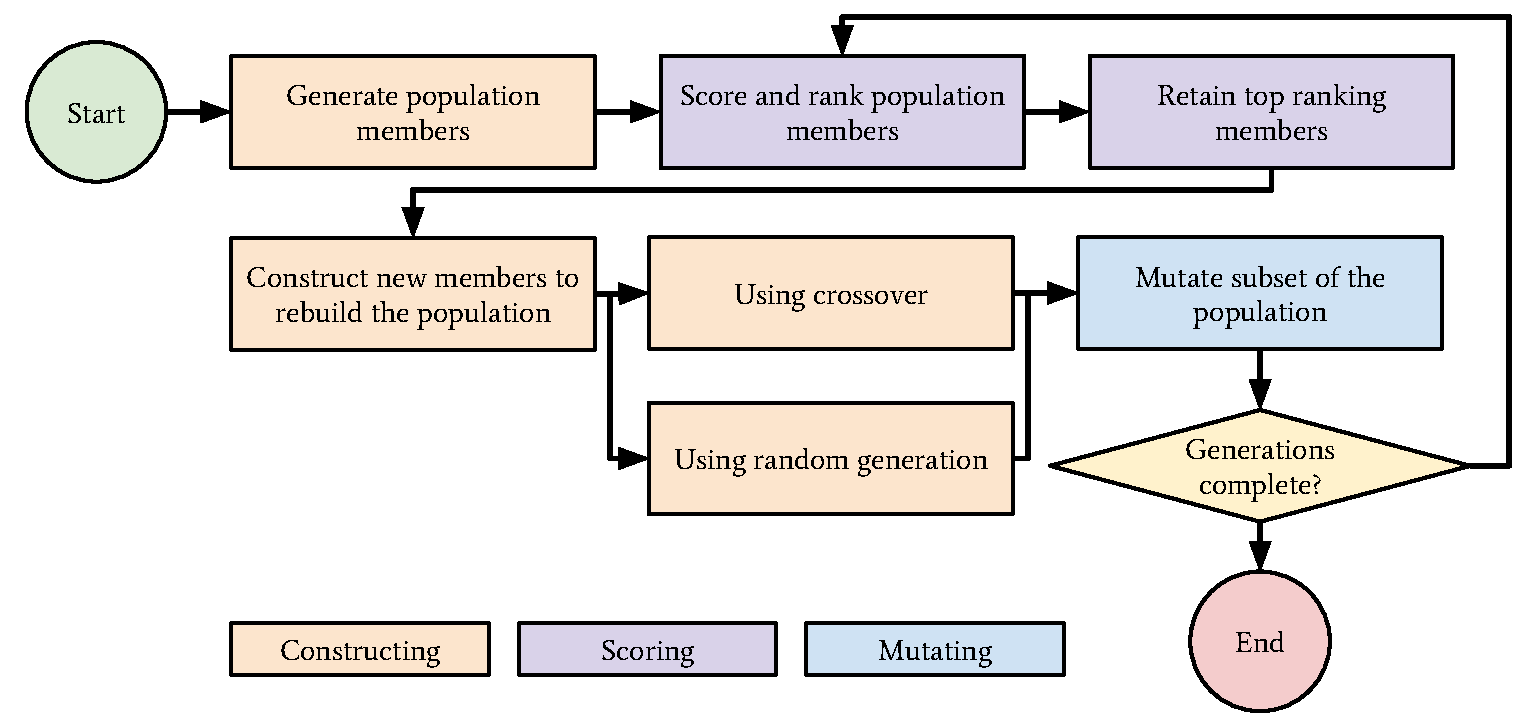
\includegraphics[width=1.0\textwidth, center]{./img/flows/ga_cycle.pdf}
    \caption{Generic genetic algorithm cycle diagram}.\label{fig:genericGACycle} 
\end{figure}

Figure~\ref{fig:genericGACycle} shows a flow diagram of a generic genetic algorithm cycle.
The specific algorithm we will be using is described in Subsection~\ref{sec:buildingTheAlgorithm}.

